\chapter{验收：数字孪生全套产品}
\label{ch:acceptance}

本章与产品验收同步产出——每一节对应一项验收，验收产生的截图/数据即书稿图源。

\section{孪生前端 v2：装配叙事与爆炸视图}
打开 \texttt{http://localhost:8000/}，首屏为装配叙事（五部件飞入合体）。
\begin{figure}[htbp]
  \centering
  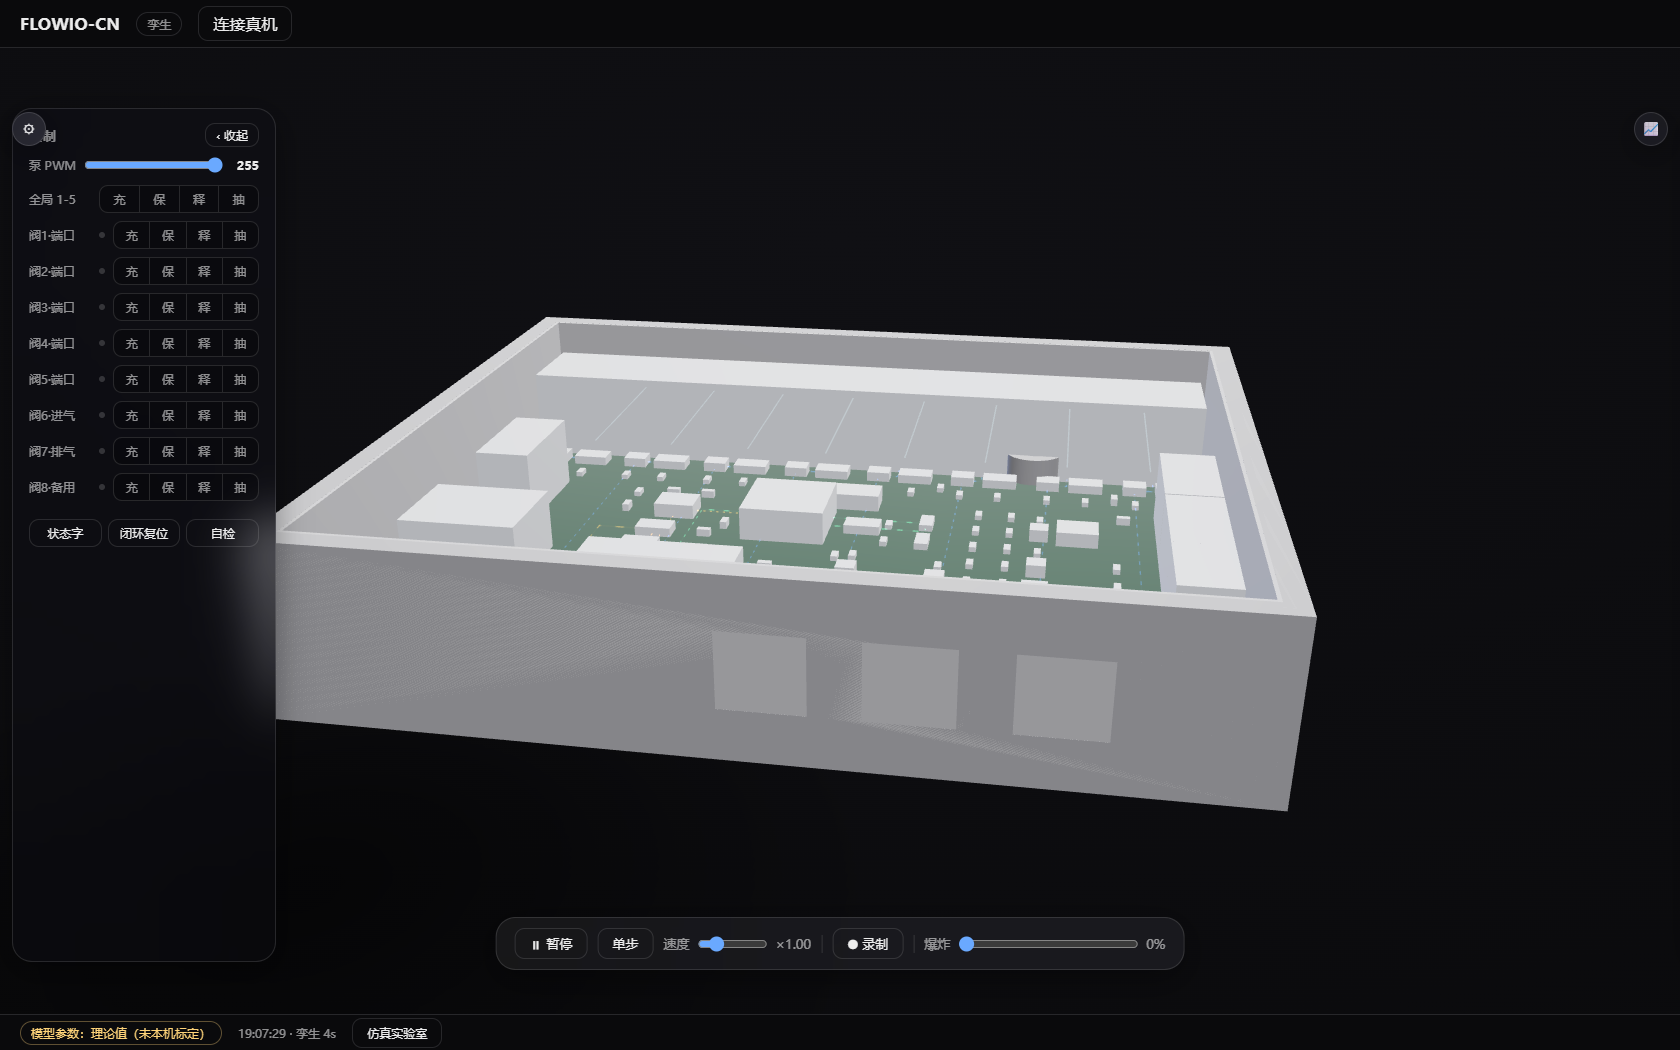
\includegraphics[width=0.9\textwidth]{figures/v2_01_intro.png}
  \caption{数字孪生 v2 首屏：产品即主角，仪表盘退居玻璃抽屉}
\end{figure}

\section{数据长在产品上：电流与气流}
发送命令 \texttt{I 1 255}（1 号端口充气），栅极支路电流辉光增强、端子喷出气流粒子：
\begin{figure}[htbp]
  \centering
  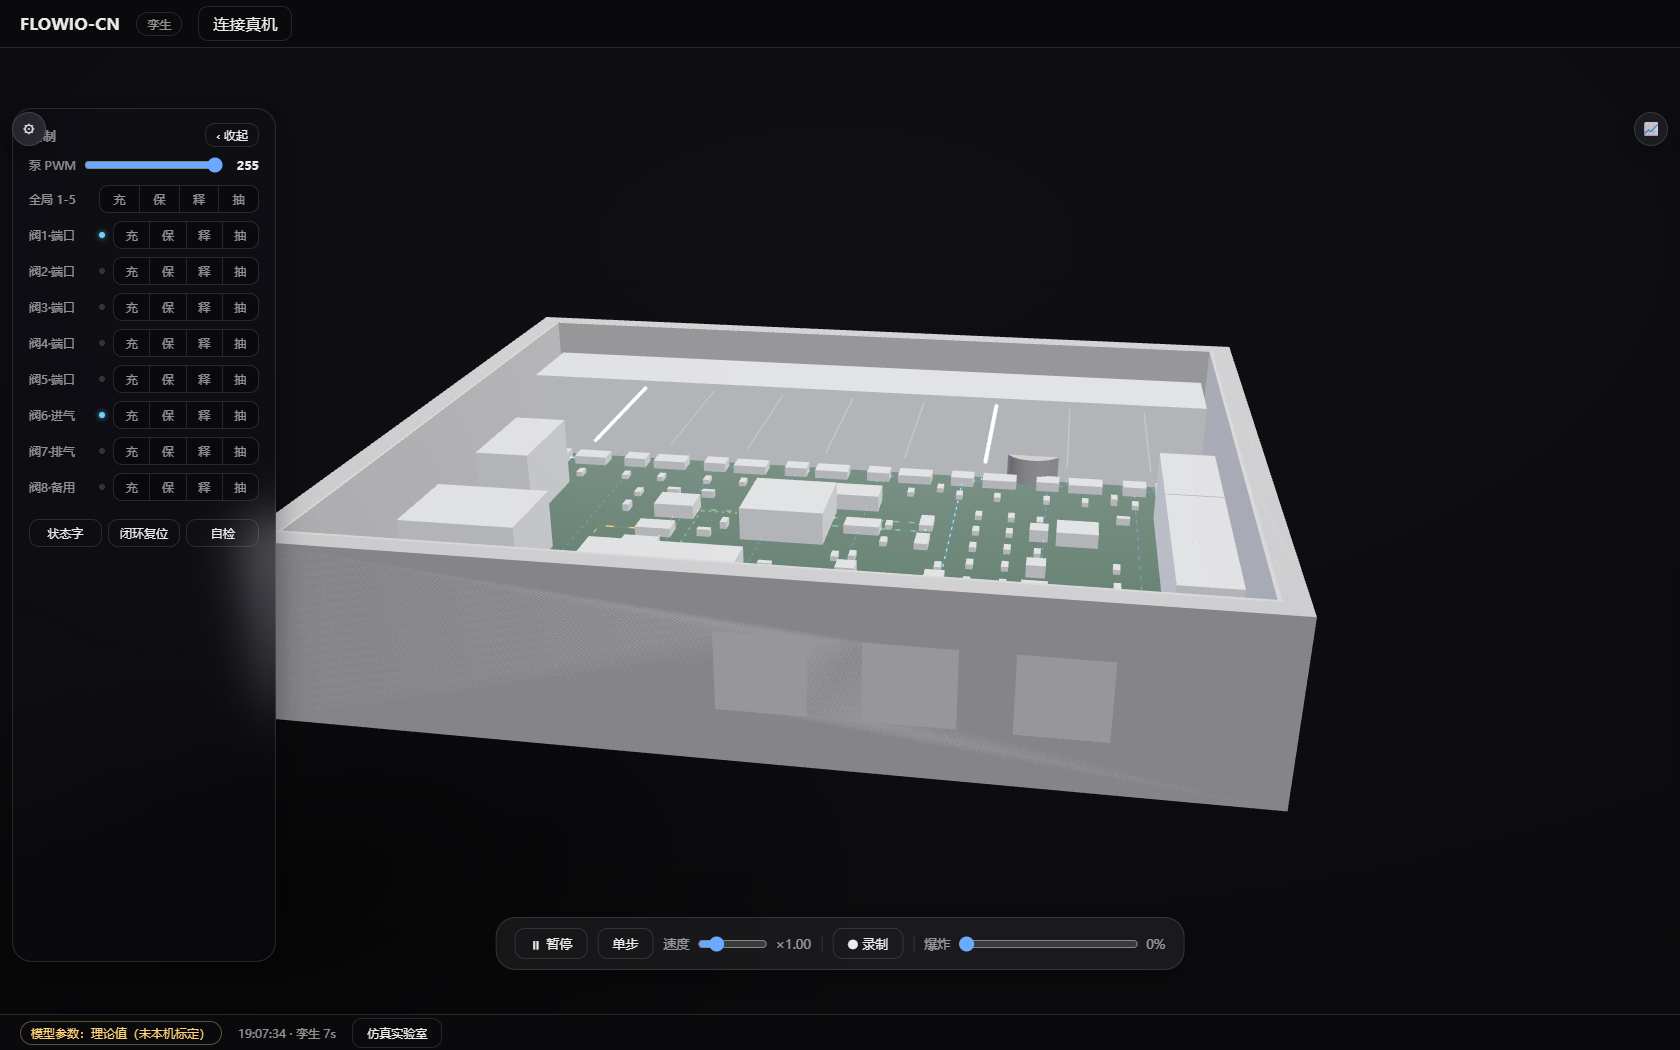
\includegraphics[width=0.9\textwidth]{figures/v2_03_inflate.png}
  \caption{充气瞬间：电流（蓝）与气流（青）由实时遥测驱动}
\end{figure}
真空模式（\texttt{V}）下气流反向并转为琥珀色（图~\ref{fig:vacuum}）。
\begin{figure}[htbp]
  \centering
  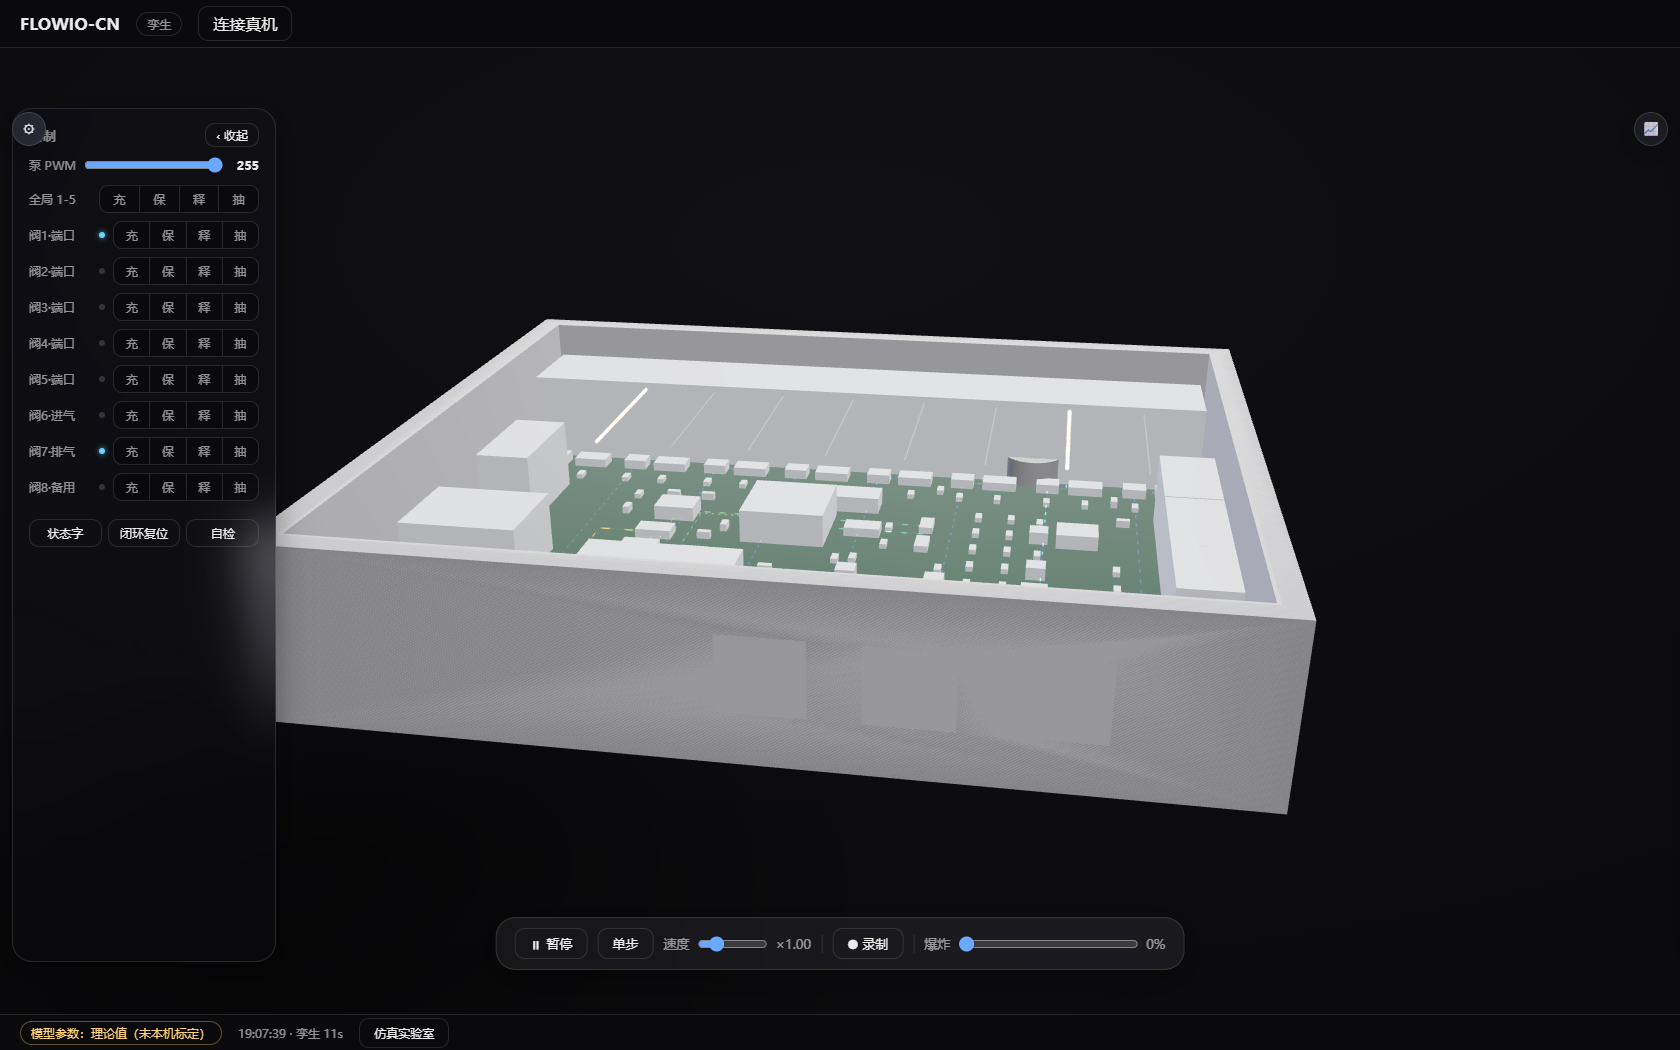
\includegraphics[width=0.9\textwidth]{figures/v2_05_vacuum.png}
  \caption{真空回流：方向与颜色随压力符号切换}\label{fig:vacuum}
\end{figure}

\section{验收清单（与 BRINGUP 联动）}
\begin{itemize}
  \item 软件侧（回板前）：装配叙事/爆炸跟随/流光联动/热点卡/仿真浮层/BLE 契约 —— 已由 44+111 断言与 26 项目视审计覆盖；
  \item 硬件侧（回板后）：按 \texttt{firmware/BRINGUP.md} 九章动线执行，产物（示波器照片/标定曲线/校准后黄徽转绿截图）直接补入本章各节。
\end{itemize}
